\documentclass[a4paper,12pt]{article} 

% First, we usually want to set the margins of our document. For this we use the package geometry.
\usepackage[top = 2.5cm, bottom = 2.5cm, left = 2.5cm, right = 2.5cm]{geometry} 
\usepackage[T1]{fontenc}
\usepackage[utf8]{inputenc}

% The following two packages - multirow and booktabs - are needed to create nice looking tables.
\usepackage{multirow} % Multirow is for tables with multiple rows within one cell.
\usepackage{booktabs} % For even nicer tables.

% As we usually want to include some plots (.pdf files) we need a package for that.
\usepackage{graphicx} 

% The default setting of LaTeX is to indent new paragraphs. This is useful for articles. But not really nice for homework problem sets. The following command sets the indent to 0.
% \usepackage{setspace}
% \setlength{\parindent}{0in}
\usepackage{indentfirst}

% Package to place figures where you want them.
\usepackage{float}

% The fancyhdr package let's us create nice headers.
\usepackage{fancyhdr}

\usepackage{xcolor,amsmath,amsthm,algorithm2e,tikz,subcaption}
\RestyleAlgo{ruled}

\definecolor{myRed}{RGB}{211, 31, 17}
\definecolor{myOrange}{RGB}{244, 122, 0}
\definecolor{myLightTeal}{RGB}{98, 200, 211}
\definecolor{myDarkTeal}{RGB}{0, 113, 145}


% To make our document nice we want a header and number the pages in the footer.

\pagestyle{fancy} % With this command we can customize the header style.

\fancyhf{} % This makes sure we do not have other information in our header or footer.

\lhead{\footnotesize Algorithm Design and Analysis(H): Assignment 2}% \lhead puts text in the top left corner. \footnotesize sets our font to a smaller size.

%\rhead works just like \lhead (you can also use \chead)
\rhead{\footnotesize Mengxuan Wu} %<---- Fill in your lastnames.

% Similar commands work for the footer (\lfoot, \cfoot and \rfoot).
% We want to put our page number in the center.
\cfoot{\footnotesize \thepage} 

\begin{document}

\thispagestyle{empty} % This command disables the header on the first page. 

\begin{tabular}{p{15.5cm}}
{\large \bf Algorithm Design and Analysis(H)} \\
Southern University of Science and Technology \\ Mengxuan Wu \\ 12212006 \\
\hline
\\
\end{tabular}

\vspace*{0.3cm} %add some vertical space in between the line and our title.

\begin{center}
	{\Large \bf Assignment 2}
	\vspace{2mm}

	{\bf Mengxuan Wu}
		
\end{center}  

\vspace*{0.4cm}

\section*{Question 1: Algorithm Description}

We introduce an efficient implementation of Edmond's algorithm for MDST problem, with the presumption that readers are familiar with the basic concepts of the algorithm.

\subsection*{Some Observations}

With observation of the algorithm, we can see that the algorithm is mainly composed of three tasks:
\begin{enumerate}
	\item find the set of minimum weight edges
	\item find the cycle in the set of minimum weight edges
	\item contract the cycle
\end{enumerate}

Among these tasks, the first one and the third one can be implemented efficiently by using a meldable heap. 
To find the minimum weight entering edge, we can simply store all entering edges of each node in a min heap.
For efficiently maintaining the heap property when contracting the cycle, we can use a meldable heap.

The second task, however, is more challenging to implement efficiently.
Finding cycle can be a time-consuming task.
In the naive implementation, when the algorithm stop to check whether the cycle is found, it checks all selected edges in the graph.
This means we may repeatedly check the same edge multiple times even if the edge is not in the cycle.

The efficient implementation we are going to introduce will focus on finding the cycle efficiently and expanding the cycles correctly.
And the other two tasks will be implemented similarly as the naive implementation, but with a more efficient data structure introduced in the following sections.

\subsection*{Finding Cycle}

As mentioned above, the cause for the inefficiency is that we may repeatedly check the same edge multiple times.
This is because after a contract operation, an edge that is not in any cycle before may become part of a cycle as figure \ref{fig:cycle} shows.

\begin{figure}[H]
	\begin{subfigure}[t]{0.5\linewidth}
		\centering
		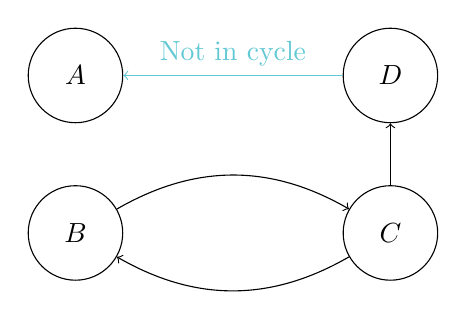
\begin{tikzpicture}
			\draw (0,0) node[draw, circle, minimum size=1.2cm] (A) {$A$};
			\draw (0,-2) node[draw, circle, minimum size=1.2cm] (B) {$B$};
			\draw (4,-2) node[draw, circle, minimum size=1.2cm] (C) {$C$};
			\draw (4,0) node[draw, circle, minimum size=1.2cm] (D) {$D$};
	
			\path[->]
			(B) edge[bend left] node {} (C)
			(C) edge[bend left] node {} (B)
			(D) edge[myLightTeal] node[above] {Not in cycle} (A)
			(C) edge node {} (D)
			;
		\end{tikzpicture}
		\caption{Before contracting the cycle}
	\end{subfigure}
	\begin{subfigure}[t]{0.5\linewidth}
		\centering
		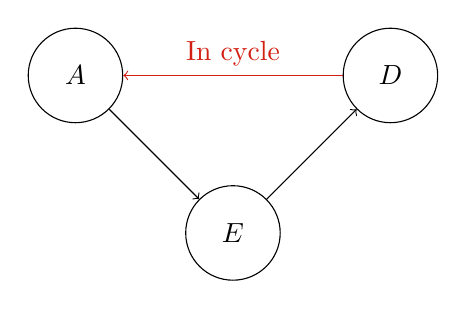
\begin{tikzpicture}
			\draw (0,0) node[draw, circle, minimum size=1.2cm] (A) {$A$};
			\draw (4,0) node[draw, circle, minimum size=1.2cm] (D) {$D$};
			\draw (2,-2) node[draw, circle, minimum size=1.2cm] (E) {$E$};
	
			\path[->]
			(D) edge[myRed] node[above] {In cycle} (A)
			(E) edge node {} (D)
			(A) edge node {} (E)
			;
		\end{tikzpicture}
		\caption{After contracting the cycle}
	\end{subfigure}
	\caption{An edge that is not in any cycle before may become part of a cycle}
	\label{fig:cycle}
\end{figure}

For this reason, every time after we contract a cycle, we still need to check all selected edges in the graph to ensure that we can find all cycles.

However, there are some observations that can help us to avoid this inefficiency.
We can find that for these nodes that are not in the cycle, their minimum weight entering edge will not change after the cycle is contracted (node $A$ and $D$ in figure \ref{fig:cycle}).
If the new cycle contains some nodes $v$ that are not in the cycle before, it means that we choose an edge $v \rightarrow s$ for the super node $s$ formed by contracting old cycle (the edge $A \rightarrow E$ in figure \ref{fig:cycle}).

Hence, the natural idea is to traverse the graph in a DFS manner by going to the starting node of the minimum weight entering edge chosen.
When we traverse the graph, we can mark the nodes as visited as we include them in the current path, and unmark them when we backtrack.
If we encounter a node that has been visited, it means that we find a cycle, and we can backtrack to identify all nodes involved and contract them.
Then we continue the DFS traversal from the newly contracted node.

In this way, we don't need to check the edges we have checked before.
Since if these edges form a cycle after some contraction, we will be able to find them again in the DFS traversal when checking the new super node.
For example, let us assume that in figure \ref{fig:cycle}, we start the DFS traversal from node $A$.
After we contract the first cycle, we continue the DFS traversal from node $E$.
Then we will find the cycle formed by the edge $A \rightarrow E$.

However, there is a problem with this approach.
With the original idea of Edmond's algorithm, we do not include the root node when we find the minimum weight entering edge for each node.
This may cause the DFS traversal starting from the root node fail to find the cycle as figure \ref{fig:fail} shows.

\begin{figure}[H]
	\centering
	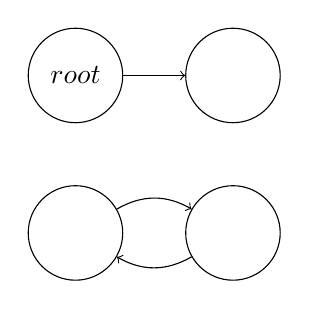
\begin{tikzpicture}
		\draw (0,0) node[draw, circle, minimum size=1.2cm] (A) {$root$};
		\draw (0,-2) node[draw, circle, minimum size=1.2cm] (B) {};
		\draw (2,-2) node[draw, circle, minimum size=1.2cm] (C) {};
		\draw (2,0) node[draw, circle, minimum size=1.2cm] (D) {};

		\path[->]
		(B) edge[bend left] node {} (C)
		(C) edge[bend left] node {} (B)
		(A) edge node {} (D)
		;
	\end{tikzpicture}
	\caption{DFS traversal starting from the root node fails to find the cycle}
	\label{fig:fail}
\end{figure}

To solve this problem, we add multiple edges to make this graph strongly connected and ignore the special treatment of the root node.
This will guarantee that the DFS traversal starting from any node will find all cycles in the graph.
However, by doing so we complicate the algorithm in two ways:
\begin{enumerate}
	\item We may choose the newly added edges in the MDST, which is not allowed.
	\item Since the graph is strongly connected, it will be contracted into a single node at the end of the algorithm.
\end{enumerate}

To solve the first problem, we add new edges with weight $\left(\sum_{v \in V} w(v)\right) + 1$.
And we can check the overall weight of the MDST at the end of the algorithm.
If the weight of the MDST is greater than $\sum_{v \in V} w(v)$, it implies that we have chosen the newly added edges in the MDST, and there is no solution to the MDST problem.
The second one is rather an advantage.
It gives us a sign that we have found the MDST, and we can stop the algorithm when only one node is left in the graph.

\subsection*{Expand Cycles}

To expand the cycles correctly, we need to maintain the information of which edge we choose for each (super) node.
This is because we avoid cycles by updating weight for all other entering edges of each involved node when contracting the cycle, instead of actually removing one edge from the cycle.
Hence, for all edges chosen there will be cycles formed by them.

With this information, we can expand the cycles with a bottom-up approach.
First, we build a contraction tree, where super nodes are parents of all nodes that are contracted to form them.
Then, we start from each node at the bottom of contraction tree, and go up to super nodes once all children are expanded.
For each node, we look at the edge we choose for it, and use this edge as the entering edge of the edge's destination node as figure \ref{fig:expand} shows.
After all nodes are expanded, we remove the entering edge of the root node, and the MDST is found.

\begin{figure}[H]
	\begin{subfigure}[t]{0.245\linewidth}
		\centering
		\resizebox{\linewidth}{!}{
			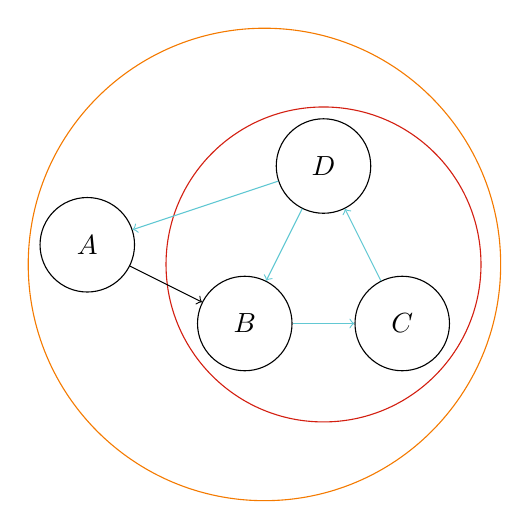
\begin{tikzpicture}
				\draw (0,0) node[draw, circle, minimum size=1.2cm] (A) {$A$};
				\draw (2,-1) node[draw, circle, minimum size=1.2cm] (B) {$B$};
				\draw (4,-1) node[draw, circle, minimum size=1.2cm] (C) {$C$};
				\draw (3,1) node[draw, circle, minimum size=1.2cm] (D) {$D$};
				\draw[myRed] (3,-0.25) circle (2cm);
				\draw[myOrange] (2.25,-0.25) circle (3cm);
		
				\path[->]
				(A) edge node {} (B)
				(B) edge[myLightTeal] node {} (C)
				(C) edge[myLightTeal] node {} (D)
				(D) edge[myLightTeal] node {} (B)
				(D) edge[myLightTeal] node {} (A)
				;
			\end{tikzpicture}
		}
		\caption{Choose edges for leaf nodes in the contraction tree first}
	\end{subfigure}
	\begin{subfigure}[t]{0.245\linewidth}
		\centering
		\resizebox{\linewidth}{!}{
		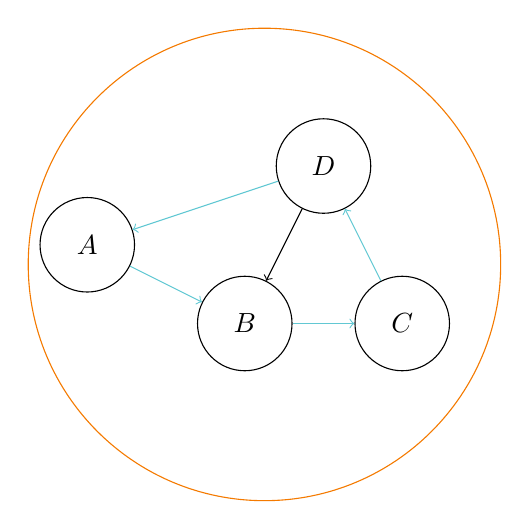
\begin{tikzpicture}
			\draw (0,0) node[draw, circle, minimum size=1.2cm] (A) {$A$};
			\draw (2,-1) node[draw, circle, minimum size=1.2cm] (B) {$B$};
			\draw (4,-1) node[draw, circle, minimum size=1.2cm] (C) {$C$};
			\draw (3,1) node[draw, circle, minimum size=1.2cm] (D) {$D$};
			\draw[myOrange] (2.25,-0.25) circle (3cm);
	
			\path[->]
			(A) edge[myLightTeal] node {} (B)
			(B) edge[myLightTeal] node {} (C)
			(C) edge[myLightTeal] node {} (D)
			(D) edge node {} (B)
			(D) edge[myLightTeal] node {} (A)
			;
		\end{tikzpicture}
		}
		\caption{Update the entering edge for $A$ and $B$ when expanding the red super node}
	\end{subfigure}
	\begin{subfigure}[t]{0.245\linewidth}
		\centering
		\resizebox{\linewidth}{!}{
		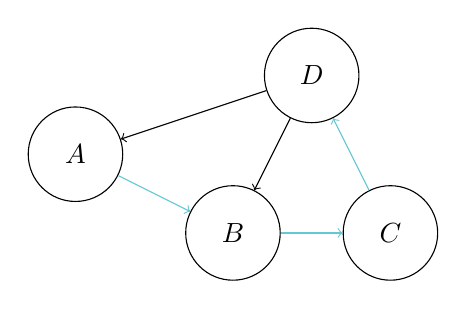
\begin{tikzpicture}
			\draw (0,0) node[draw, circle, minimum size=1.2cm] (A) {$A$};
			\draw (2,-1) node[draw, circle, minimum size=1.2cm] (B) {$B$};
			\draw (4,-1) node[draw, circle, minimum size=1.2cm] (C) {$C$};
			\draw (3,1) node[draw, circle, minimum size=1.2cm] (D) {$D$};
	
			\path[->]
			(A) edge[myLightTeal] node {} (B)
			(B) edge[myLightTeal] node {} (C)
			(C) edge[myLightTeal] node {} (D)
			(D) edge node {} (B)
			(D) edge node {} (A)
			;
		\end{tikzpicture}
		}
		\caption{Remove the entering edge for root node $A$ when expanding the final orange super node}
	\end{subfigure}
	\begin{subfigure}[t]{0.245\linewidth}
		\centering
		\resizebox{\linewidth}{!}{
			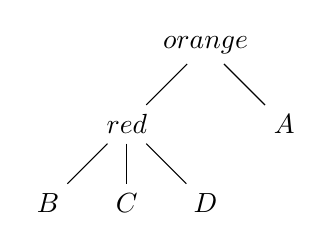
\begin{tikzpicture}
				\draw (0,0) node (orange) {$orange$};
				\draw (-1,-1) node (red) {$red$};
				\draw (1,-1) node (A) {$A$};
				\draw (-2,-2) node (B) {$B$};
				\draw (-1,-2) node (C) {$C$};
				\draw (0,-2) node (D) {$D$};

				\path
				(orange) edge node {} (red)
				(orange) edge node {} (A)
				(red) edge node {} (B)
				(red) edge node {} (C)
				(red) edge node {} (D)
				;
			\end{tikzpicture}
		}
		\caption{Contraction tree}
	\end{subfigure}
	\caption{Expand cycles with a bottom-up approach}
	\label{fig:expand}
\end{figure}

\section*{Question 2: Meldable Heap}

For task 1 and task 3, we need a data structure that can efficiently carry out the following operations:
\begin{enumerate}
	\item Find the minimum element
	\item reduce all elements by a constant
	\item meld two of these into one
\end{enumerate}

It is natural to use a heap for operation 1.
But an array-based heap is slow for other two operations.
We will need to traverse all elements in the heap, and the tree structure of the heap is not utilized.

A better choice is to use a heap based on pointers instead of arrays, which allows us to utilize the tree structure of the heap.
We will introduce the leftist tree as the data structure for the heap.

\subsection*{Leftist Tree Definition}

We first define the distance of each node in the leftist tree as follows:
\begin{itemize}
	\item A node the has no children has $n.dist = -1$.
	\item A node that has only one child has $n.dist = 0$.
	\item A node that has two children has $n.dist = \min(n.left.dist, n.right.dist) + 1$.
\end{itemize}

The leftist tree is a binary tree that satisfies the leftist property:
The distance of the left child is greater than or equal to the distance of the right child.
And for this reason, we can always find $n.dist = n.right.dist + 1$ in a leftist tree.

By this property, a leftist tree with $n$ nodes has a distance of at most $\lceil \log (n+1) \rceil - 2$ for its root node.
\begin{proof}
$ $

We proof this by induction.

\textbf{Base case:} 

For a root node whose $dist =  -1$, the minimum number of node that can be in the tree is 1, which is the root node.
For a root node whose $dist = 0$, the minimum number of node that can be in the tree is 3, which is the root node and its two children.

\textbf{Inductive step:}
For a root node whose $dist = k \geq 1$, we can see that if we want the tree to have the minimum number of nodes, both left and right child should have distance $k-1$ and should be the minimum tree of that distance.
Hence, the minimum tree will be a full binary tree.
And we can draw the conclusion easily.
\end{proof}

\subsection*{Leftist Tree Operations}

\subsubsection*{Merge}

The most important operation of the leftist tree is the merge operation.
It takes two leftist trees and merges them into one leftist tree.
The merge operation is defined as algorithm \ref{algo:merge}.

The merge operation is a recursive operation.
It first compares the root of two trees, and choose the smaller one as the root of the new tree.
Then it recursively merges the right child of the tree with the other tree.
After the merge operation, it swaps the left and right child if the distance of the left child is less than the distance of the right child, to maintain the leftist property.

\begin{algorithm}[H]
	\caption{Merge}
	\label{algo:merge}
	\KwIn{Two leftist trees $T_1$ and $T_2$}
	\KwOut{A leftist tree that contains all elements in $T_1$ and $T_2$}
	\If{$T_1$ is empty}{
		\Return $T_2$\;
	}
	\If{$T_2$ is empty}{
		\Return $T_1$\;
	}
	\If{The root of $T_1$ is greater than the root of $T_2$}{
		Swap $T_1$ and $T_2$\;
	}
	$T_1.right \leftarrow Merge(T_1.right, T_2)$\;
	\If{The distance of $T_1.left$ is less than the distance of $T_1.right$}{
		Swap $T_1.left$ and $T_1.right$\;
	}
	\Return $T_1$\;
\end{algorithm}

The key idea of the merge operation is that we always recursively merge the right child of the tree.
Since the property mentioned above, one of the trees' distance will be reduced by 1 after each merge operation.
And the merge operation will stop once one of the tree is empty.
Hence, we can guarantee the merge operation takes $O(\log n + \log m)$ time, where $n$ and $m$ are the number of nodes originally in $T_1$ and $T_2$ respectively.

In the leftist tree, most operations are replaced by the merge operation.
For example, to insert an element, we can merge the tree with a single node with the tree.
To delete the minimum element, we can merge the left and right child of the root node.

\subsubsection*{Pushdown}

When we need to reduce all elements in the leftist tree by a constant, we can use the pushdown operation.
Since adding, reducing all elements in a heap by a constant will not change the order of the elements, we don't need to update the key of each element until it needs to be compared in the merge operation.
We do this by adding a tag to each node, which represents the constant we need to reduce for all of its children.
When we need to compare the key of a node, we first reduce the key by the tag of the node, add this tag to the children of the node, and reset the tag of current node to 0.

\begin{center}
	\resizebox{0.85\linewidth}{!}{
		\begin{algorithm}[H]
			\caption{Pushdown operation}
			\KwIn{A node $n$}
			\If{$n$ is not empty}{
				\If{$n.left$ is not empty}{
					$n.left.tag \leftarrow n.left.tag + n.tag$\;
					$n.left.key \leftarrow n.left.key - n.tag$\;
				}
				\If{$n.right$ is not empty}{
					$n.right.tag \leftarrow n.right.tag + n.tag$\;
					$n.right.key \leftarrow n.right.key - n.tag$\;
				}
				$n.tag \leftarrow 0$\;
			}
		\end{algorithm}
	}
\end{center}

\begin{center}
	\resizebox{0.85\linewidth}{!}{
		\begin{algorithm}[H]
			\caption{Merge with pushdown}
			\KwIn{Two leftist trees $T_1$ and $T_2$}
			\KwOut{A leftist tree that contains all elements in $T_1$ and $T_2$}
			\If{$T_1$ is empty}{
				\Return $T_2$\;
			}
			\If{$T_2$ is empty}{
				\Return $T_1$\;
			}
			Pushdown($T_1.root$)\;
			Pushdown($T_2.root$)\;
			\If{The root of $T_1$ is greater than the root of $T_2$}{
				Swap $T_1$ and $T_2$\;
			}
			$T_1.right \leftarrow Merge(T_1.right, T_2)$\;
			\If{The distance of $T_1.left$ is less than the distance of $T_1.right$}{
				Swap $T_1.left$ and $T_1.right$\;
			}
			\Return $T_1$\;
		\end{algorithm}
	}
\end{center}

\section*{Question 3: Time Complexity Analysis}

The full algorithm is defined as algorithm \ref{algo:mdst}.

\begin{center}
	\resizebox{0.85\linewidth}{!}{
	\begin{algorithm}[H]
		\caption{MDST}
		\label{algo:mdst}
		\KwIn{A graph $G = (V, E)$, a root node $r$}
		\KwOut{The minimum directed spanning tree of $G$ rooted at $r$}
		\For{$i$ from 1 to $|V|$}{
			$E.add(v_i, v_{i+1}, \sum_{v \in V} w(v) + 1)$\; 
		}
		\ForEach{$e \in E$}{
			$leftistTree[e.destination].push(e)$\;
		}
		$S \gets$ empty stack\;
		$S.push(r)$\;
		\While{leftistTree[S.top] is not empty}{
			$e \gets leftistTree[S.top].pop()$\;
			\If{$e.destination$ is in the same super node as $e.source$}{
				continue\;
			}
			\If{$visited[e.destination] = false$}{
				$visited[e.destination] \gets true$\;
				$S.push(e.destination)$\;
				continue\;
			}
			super node $s \gets$ new node\;
			\While{$visited[e.source] = true$}{
				assign $S.top$ to $s$\;
				reduce all entering edges of $S.top$ by $leftistTree[S.top].min()$\;
				$leftistTree[S.top].pop()$\;
				meld $leftistTree[S.top]$ with $leftistTree[s]$\;
				$visited[S.top] \gets false$\;
				$S.pop()$\;
			}
		}
	\end{algorithm}
	}
\end{center}

When we contract a cycle, we need to meld all nodes in the cycle.
Since there are at most $|V|$ nodes in the graph, we need to do at most $|V|-1$ meld operations.
For each node, we at most have $|V| - 1$ entering edges in the heap (duplicate edges can be removed and keep only the minimum weight edge).
For this part, the time complexity is $O((|V| - 1) \log (|V| - 1))$.

Also, we need to pop each edge in the heap.
Similarly, we need to do $|E|$ pop operations, and each pop operation takes $O(\log (|V| - 1))$ time.
Hence, the time complexity for this part is $O(|E| \log (|V| - 1))$.

The overall time complexity of the algorithm is $O((|E| + |V|) \log |V|)$ or simply $O(|E| \log |V|)$, which is equivalent to $O(m \log n)$.

\section*{Question 4: Space Complexity Analysis}

The leftist tree will be taking most of the space.
We need to store each edge as a node in the leftist tree, and also add $|V|$ new edges to the graph to make it strongly connected.
Hence, there will be at most $|E| + |V|$ nodes in the leftist tree.
Other parts of the algorithm are about storing information about each (super) node, which takes $O(2|V|)$ space.

Hence, the space complexity of the algorithm is $O(|E| + |V|)$, which is equivalent to $O(m + n)$.

\end{document}